
The Bode plot of the altitude loop $P_{lon}(s)$ and the loop gain  with PID control $P_{lon}(s)C_{PID}(s)$,are shown in Figure~\ref{fig:hw_vtol_alt_bode_specs}.
\begin{figure}[H]
   \centering
   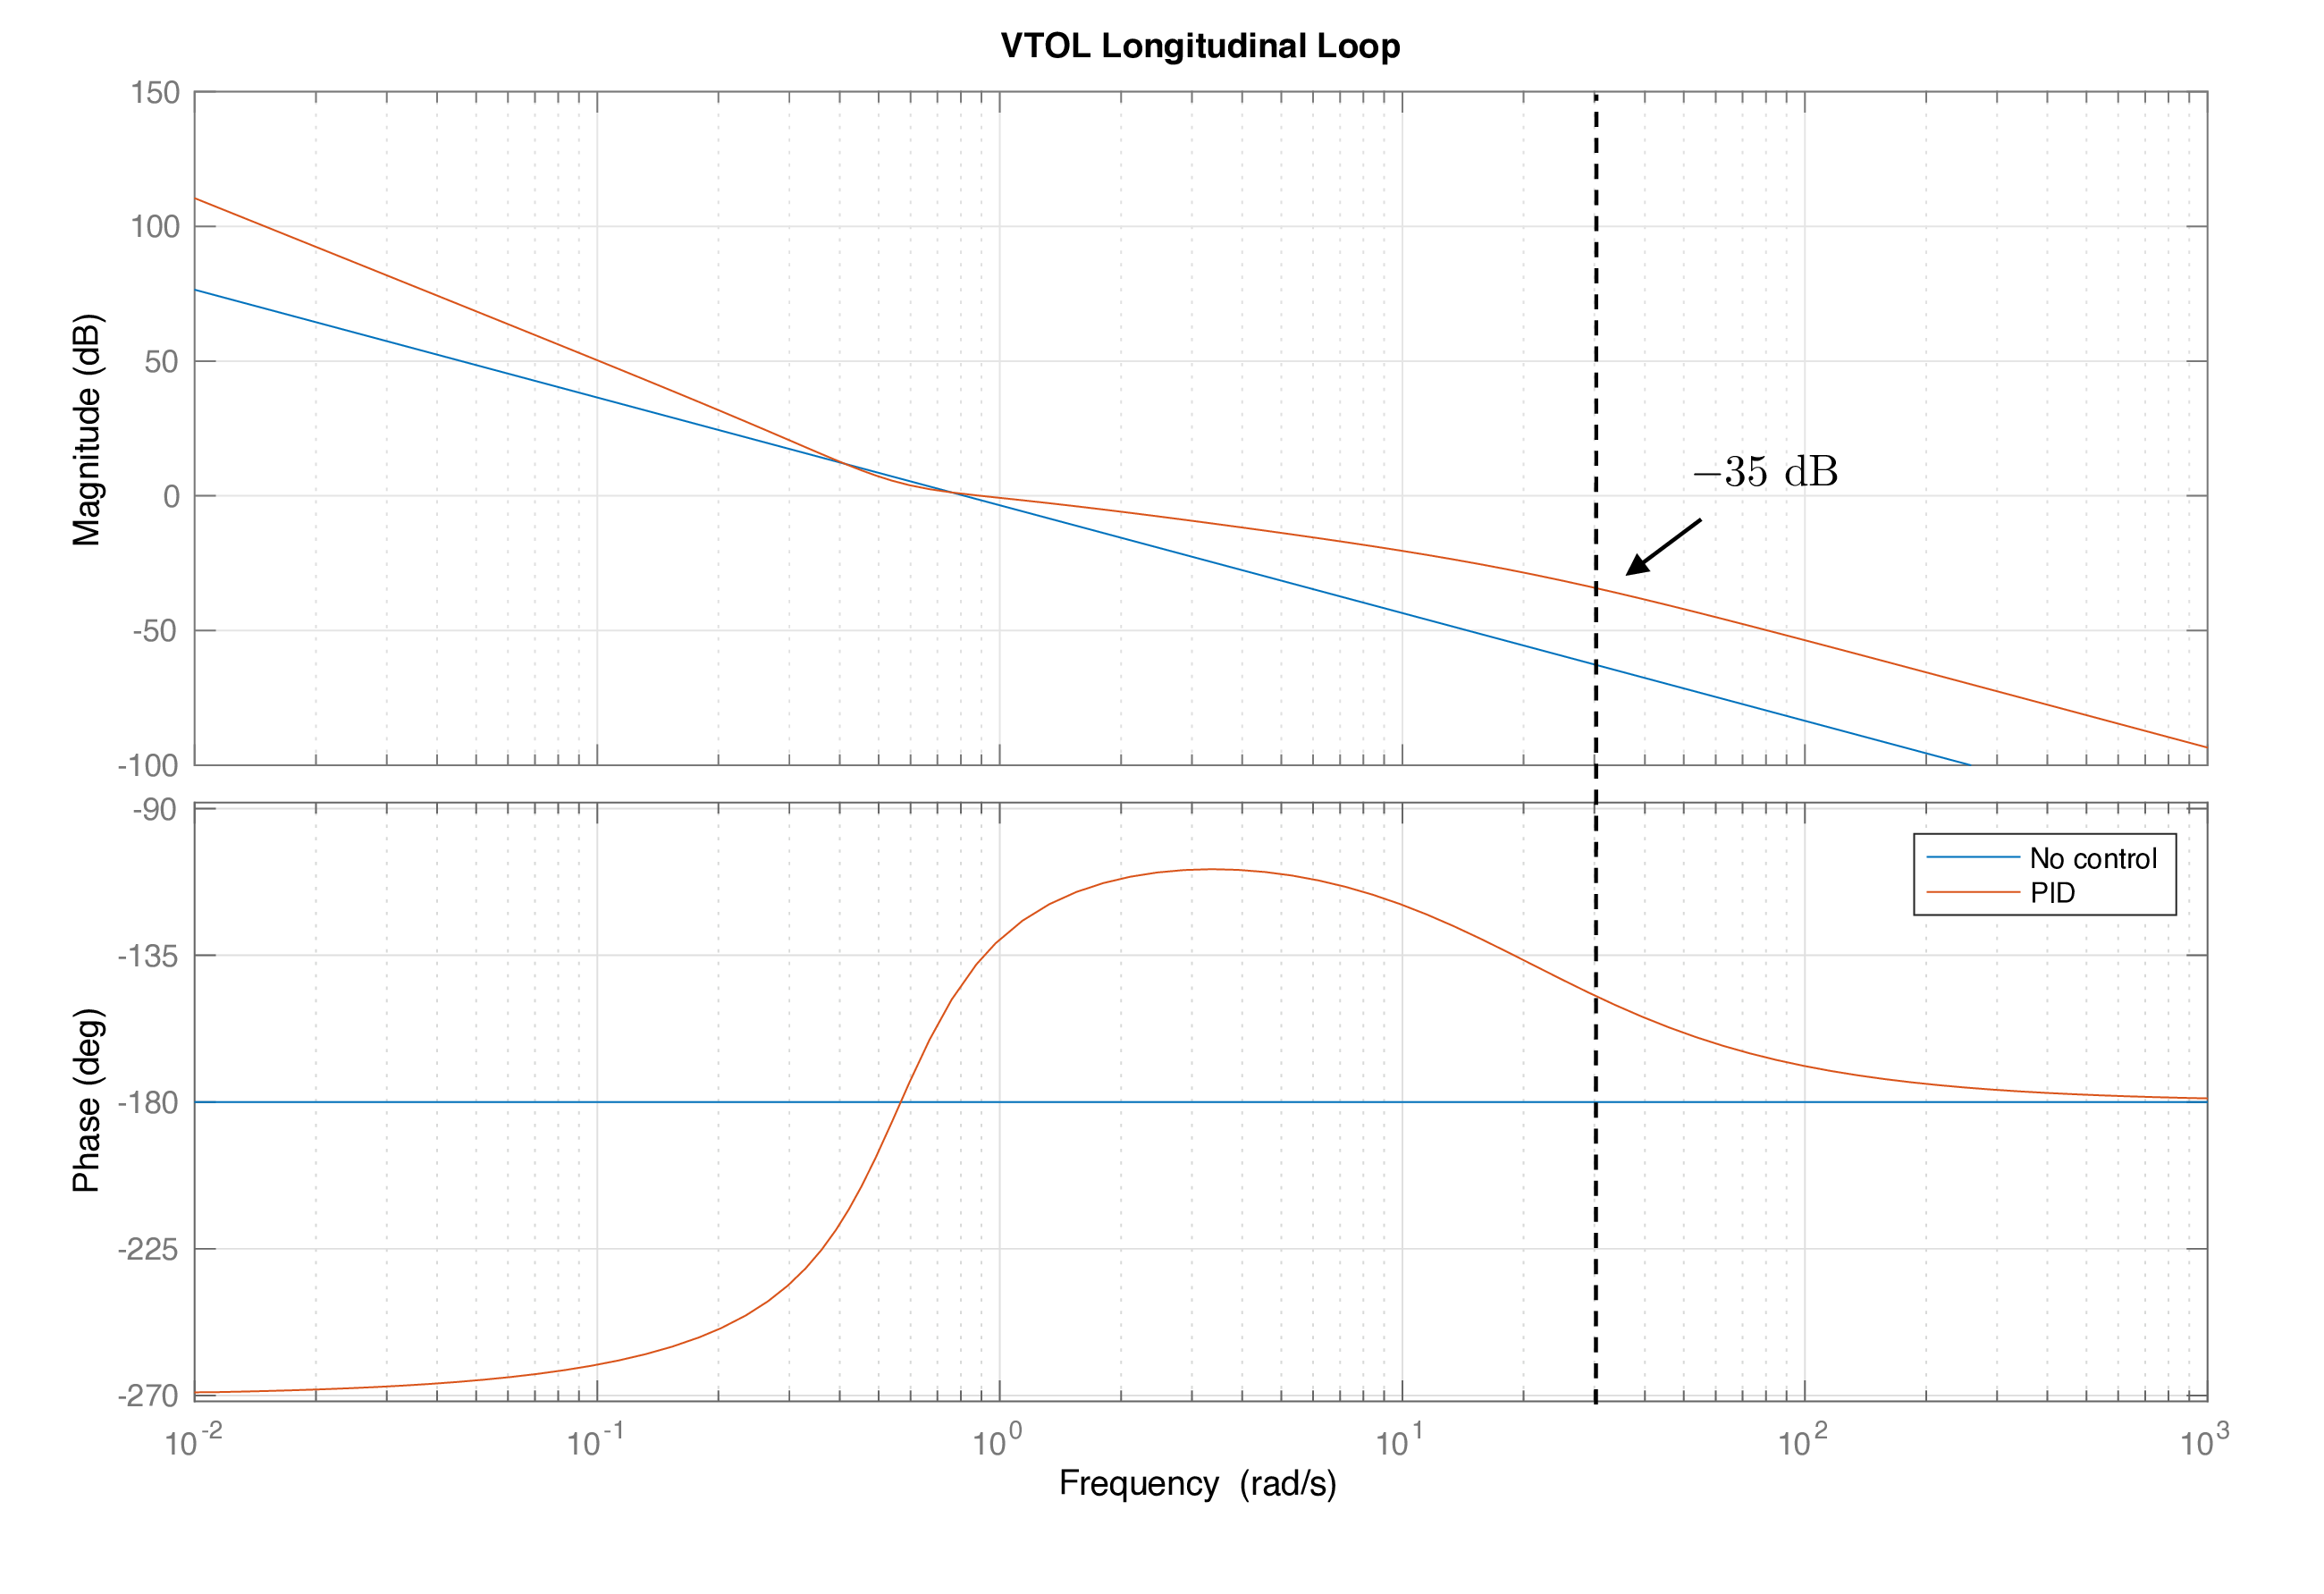
\includegraphics[width=0.95\textwidth]{6_design_studies/figures/hw_vtol_alt_bode_specs.pdf}
   \caption{Bode plot for altitude loop of the VTOL system, plant only and under PID control.}
   \label{fig:hw_vtol_alt_bode_specs}
\end{figure}

{\bf (a)}
For PID control, the slope of the Bode plot is $-60$~dB/dec as $\omega\to 0$.  Therefore, the system is type~3 and will track a parabola with zero steady state error. 

{\bf (b)} For $\omega\geq\omega_{no}=30$~rad/sec, we see from Figure~\ref{fig:hw_vtol_alt_bode_specs} that $B_{no} = -35$~dB.  Therefore, $\gamma_n = 10^{-35/20} = 0.0178$ which implies that $1.78$\% of the noise will show up in the output signal.

The Bode plot of the lateral inner loop $P_{lat,in}(s)$, and the loop gain with PD control $P_{lat,in}(s)C_{PD}(s)$, are shown in Figure~\ref{fig:hw_vtol_lat_bode_specs_in}.
\begin{figure}[H]
   \centering
   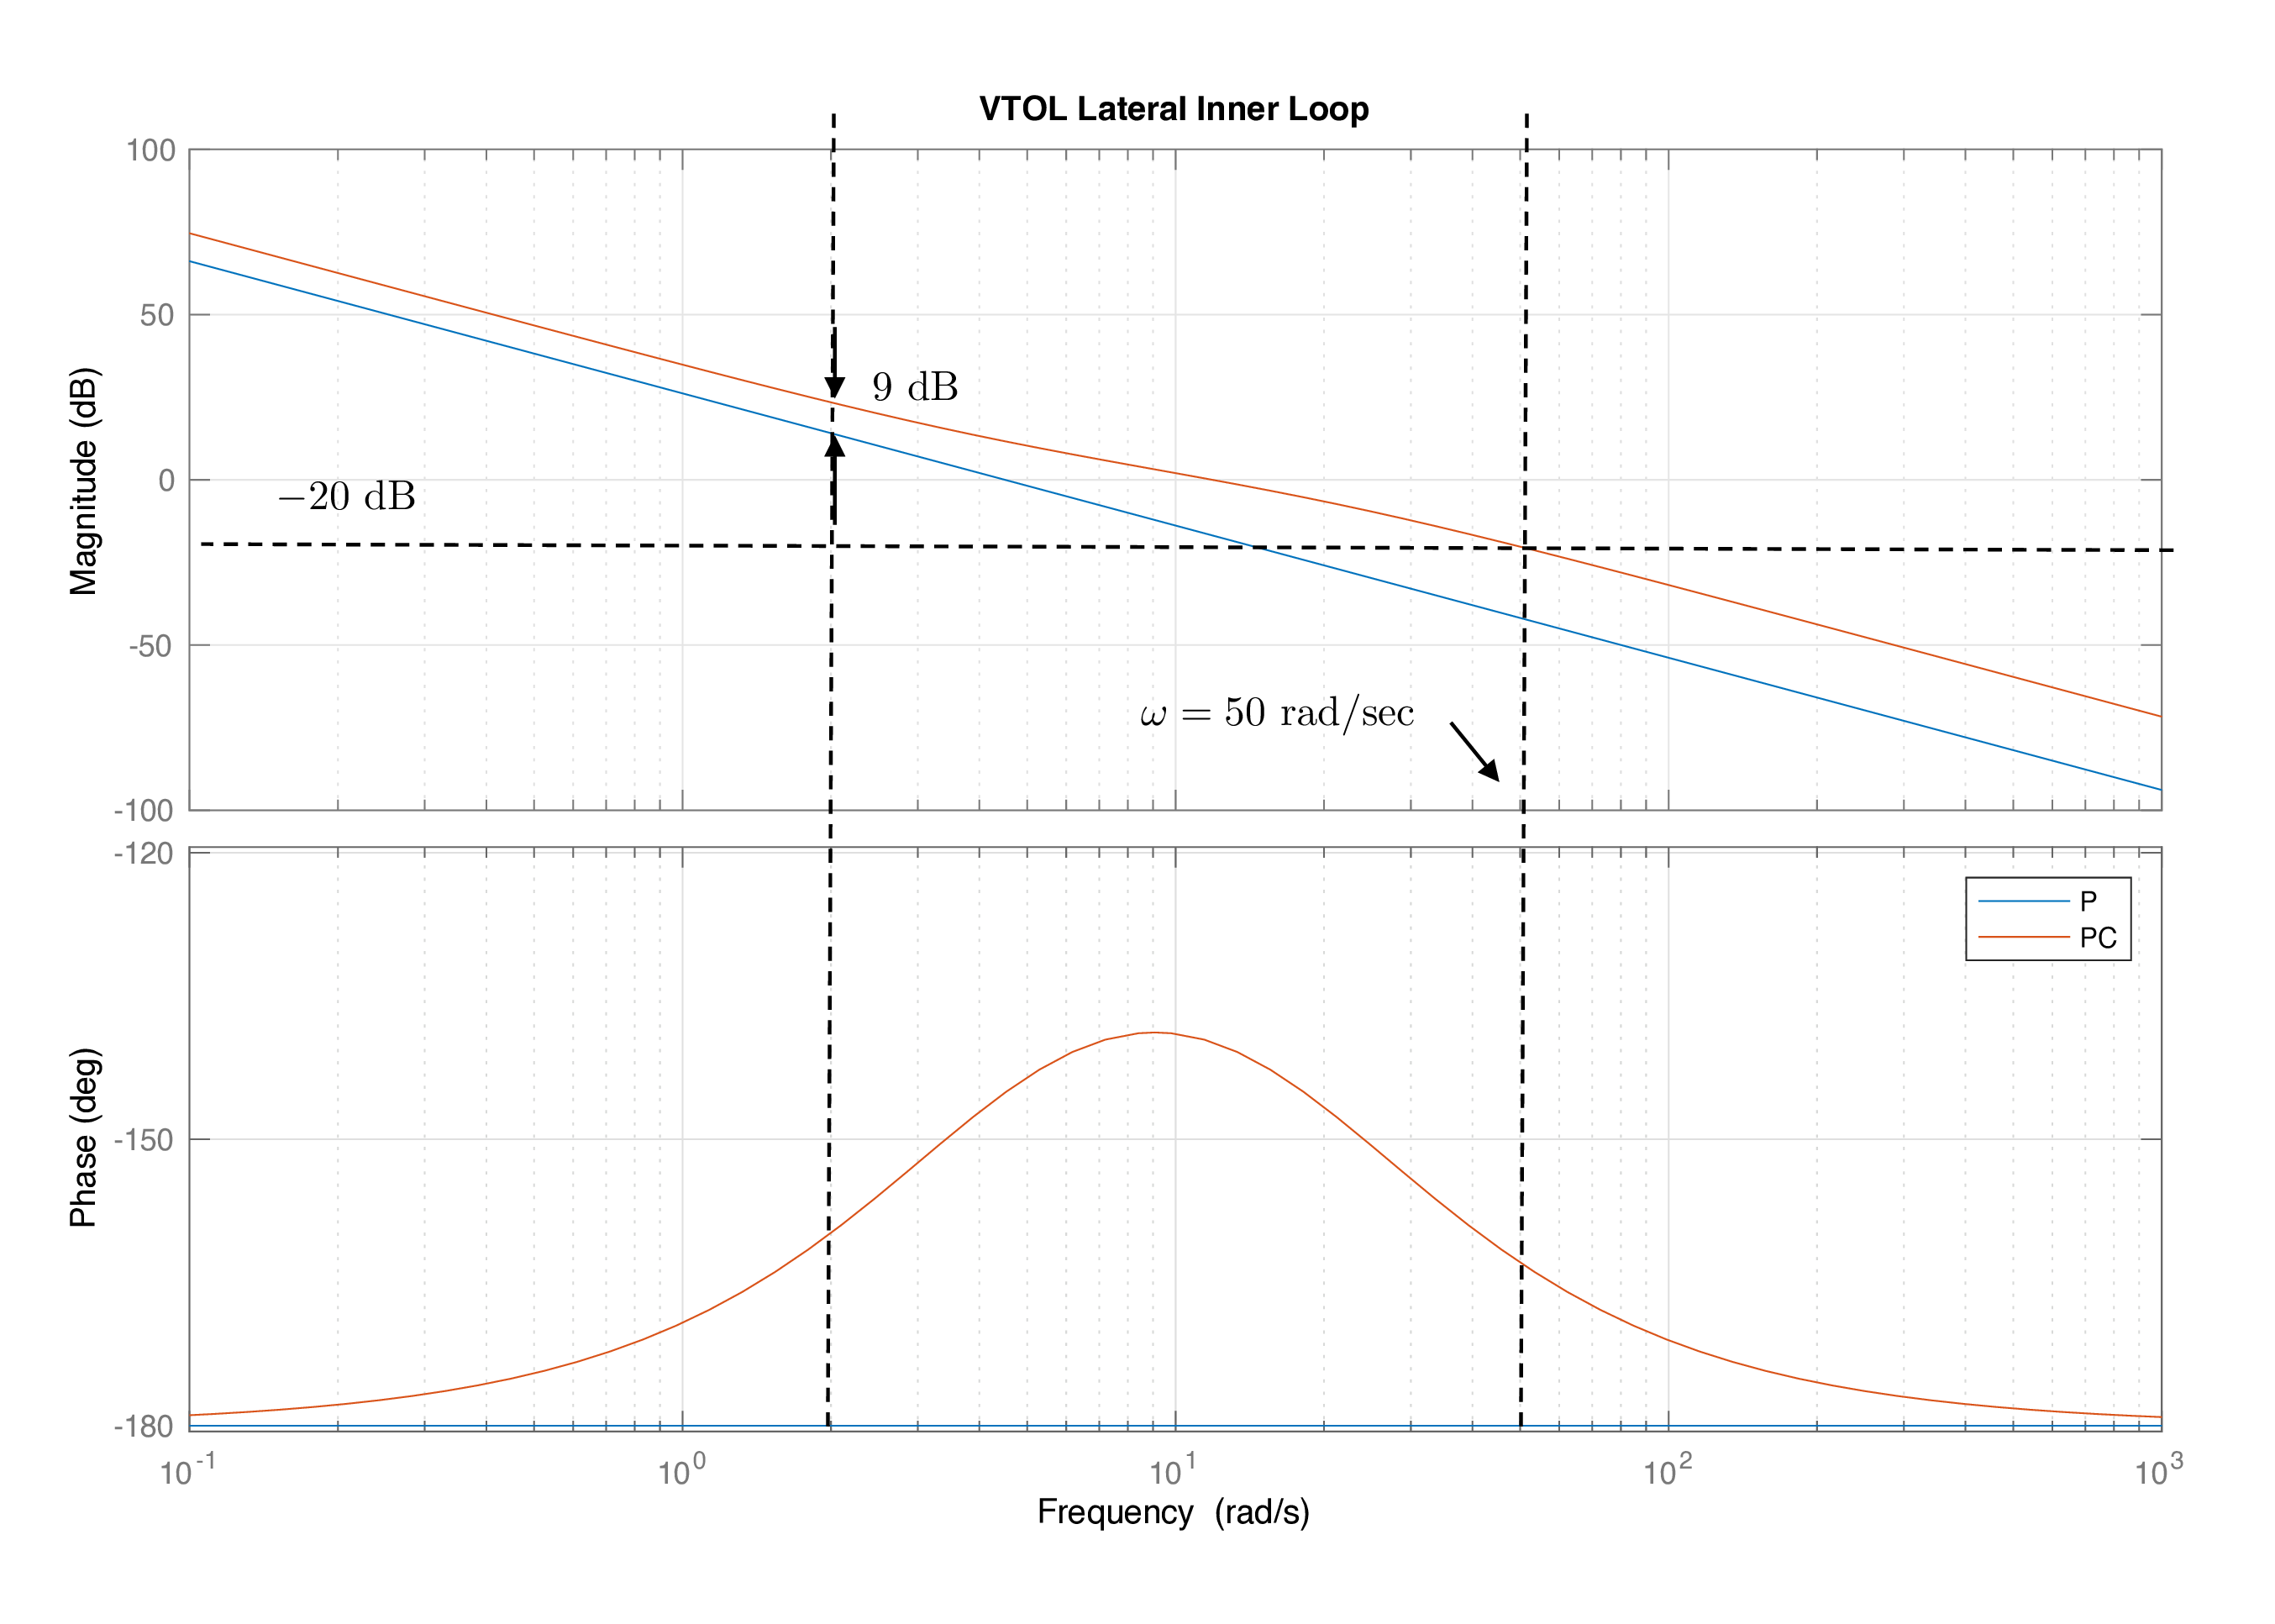
\includegraphics[width=0.95\textwidth]{6_design_studies/figures/hw_vtol_lat_bode_specs_in.pdf}
   \caption{Bode plot for lateral inner loop of the VTOL system, plant only, and under PD control.}
   \label{fig:hw_vtol_lat_bode_specs_in}
\end{figure}

{\bf (c)}
From Figure~\ref{fig:hw_vtol_lat_bode_specs_in} we see that for $\omega\leq\omega_{d_{in}}=2$~dB, the Bode magnitude plot satisfies 
\[
20\log_{10}\abs{P(j\omega)C(j\omega)}-20\log_{10}\abs{P(j\omega)} \geq B_{d_{in}}=9\text{~dB}.
\]  
Therefore, the contribution of the input disturbance to the error satisfies
\[
\abs{e(t)} \leq 10^{-9/20}\abs{d_{in}(t)} = 0.3548\abs{d_{in}(t)},
\]
which implies that $35$\% of the input disturbance shows up in the output $\theta$.

{\bf (d)}
For an error of $0.1$~degrees we need 
\[
\abs{y(t)}\leq 10^{B_{no}/20}\abs{n(t)} = 0.1 \text{~degrees} 
\]
If the sensor can produce $1$~degree of noise, then we need $B_{no}=-20$~dB.  From Figure~\ref{fig:hw_vtol_lat_bode_specs_in} this would require that the frequency content of the noise should be greater than or equal to $\omega_n=50$~rad/sec.

The Bode plot of the lateral outer loop $P_{lat,out}(s)$, and the loop gain with PD control $P_{lat,out}(s)C_{PD}(s)$, are shown in Figure~\ref{fig:hw_vtol_lat_bode_specs_out}.
\begin{figure}[H]
   \centering
   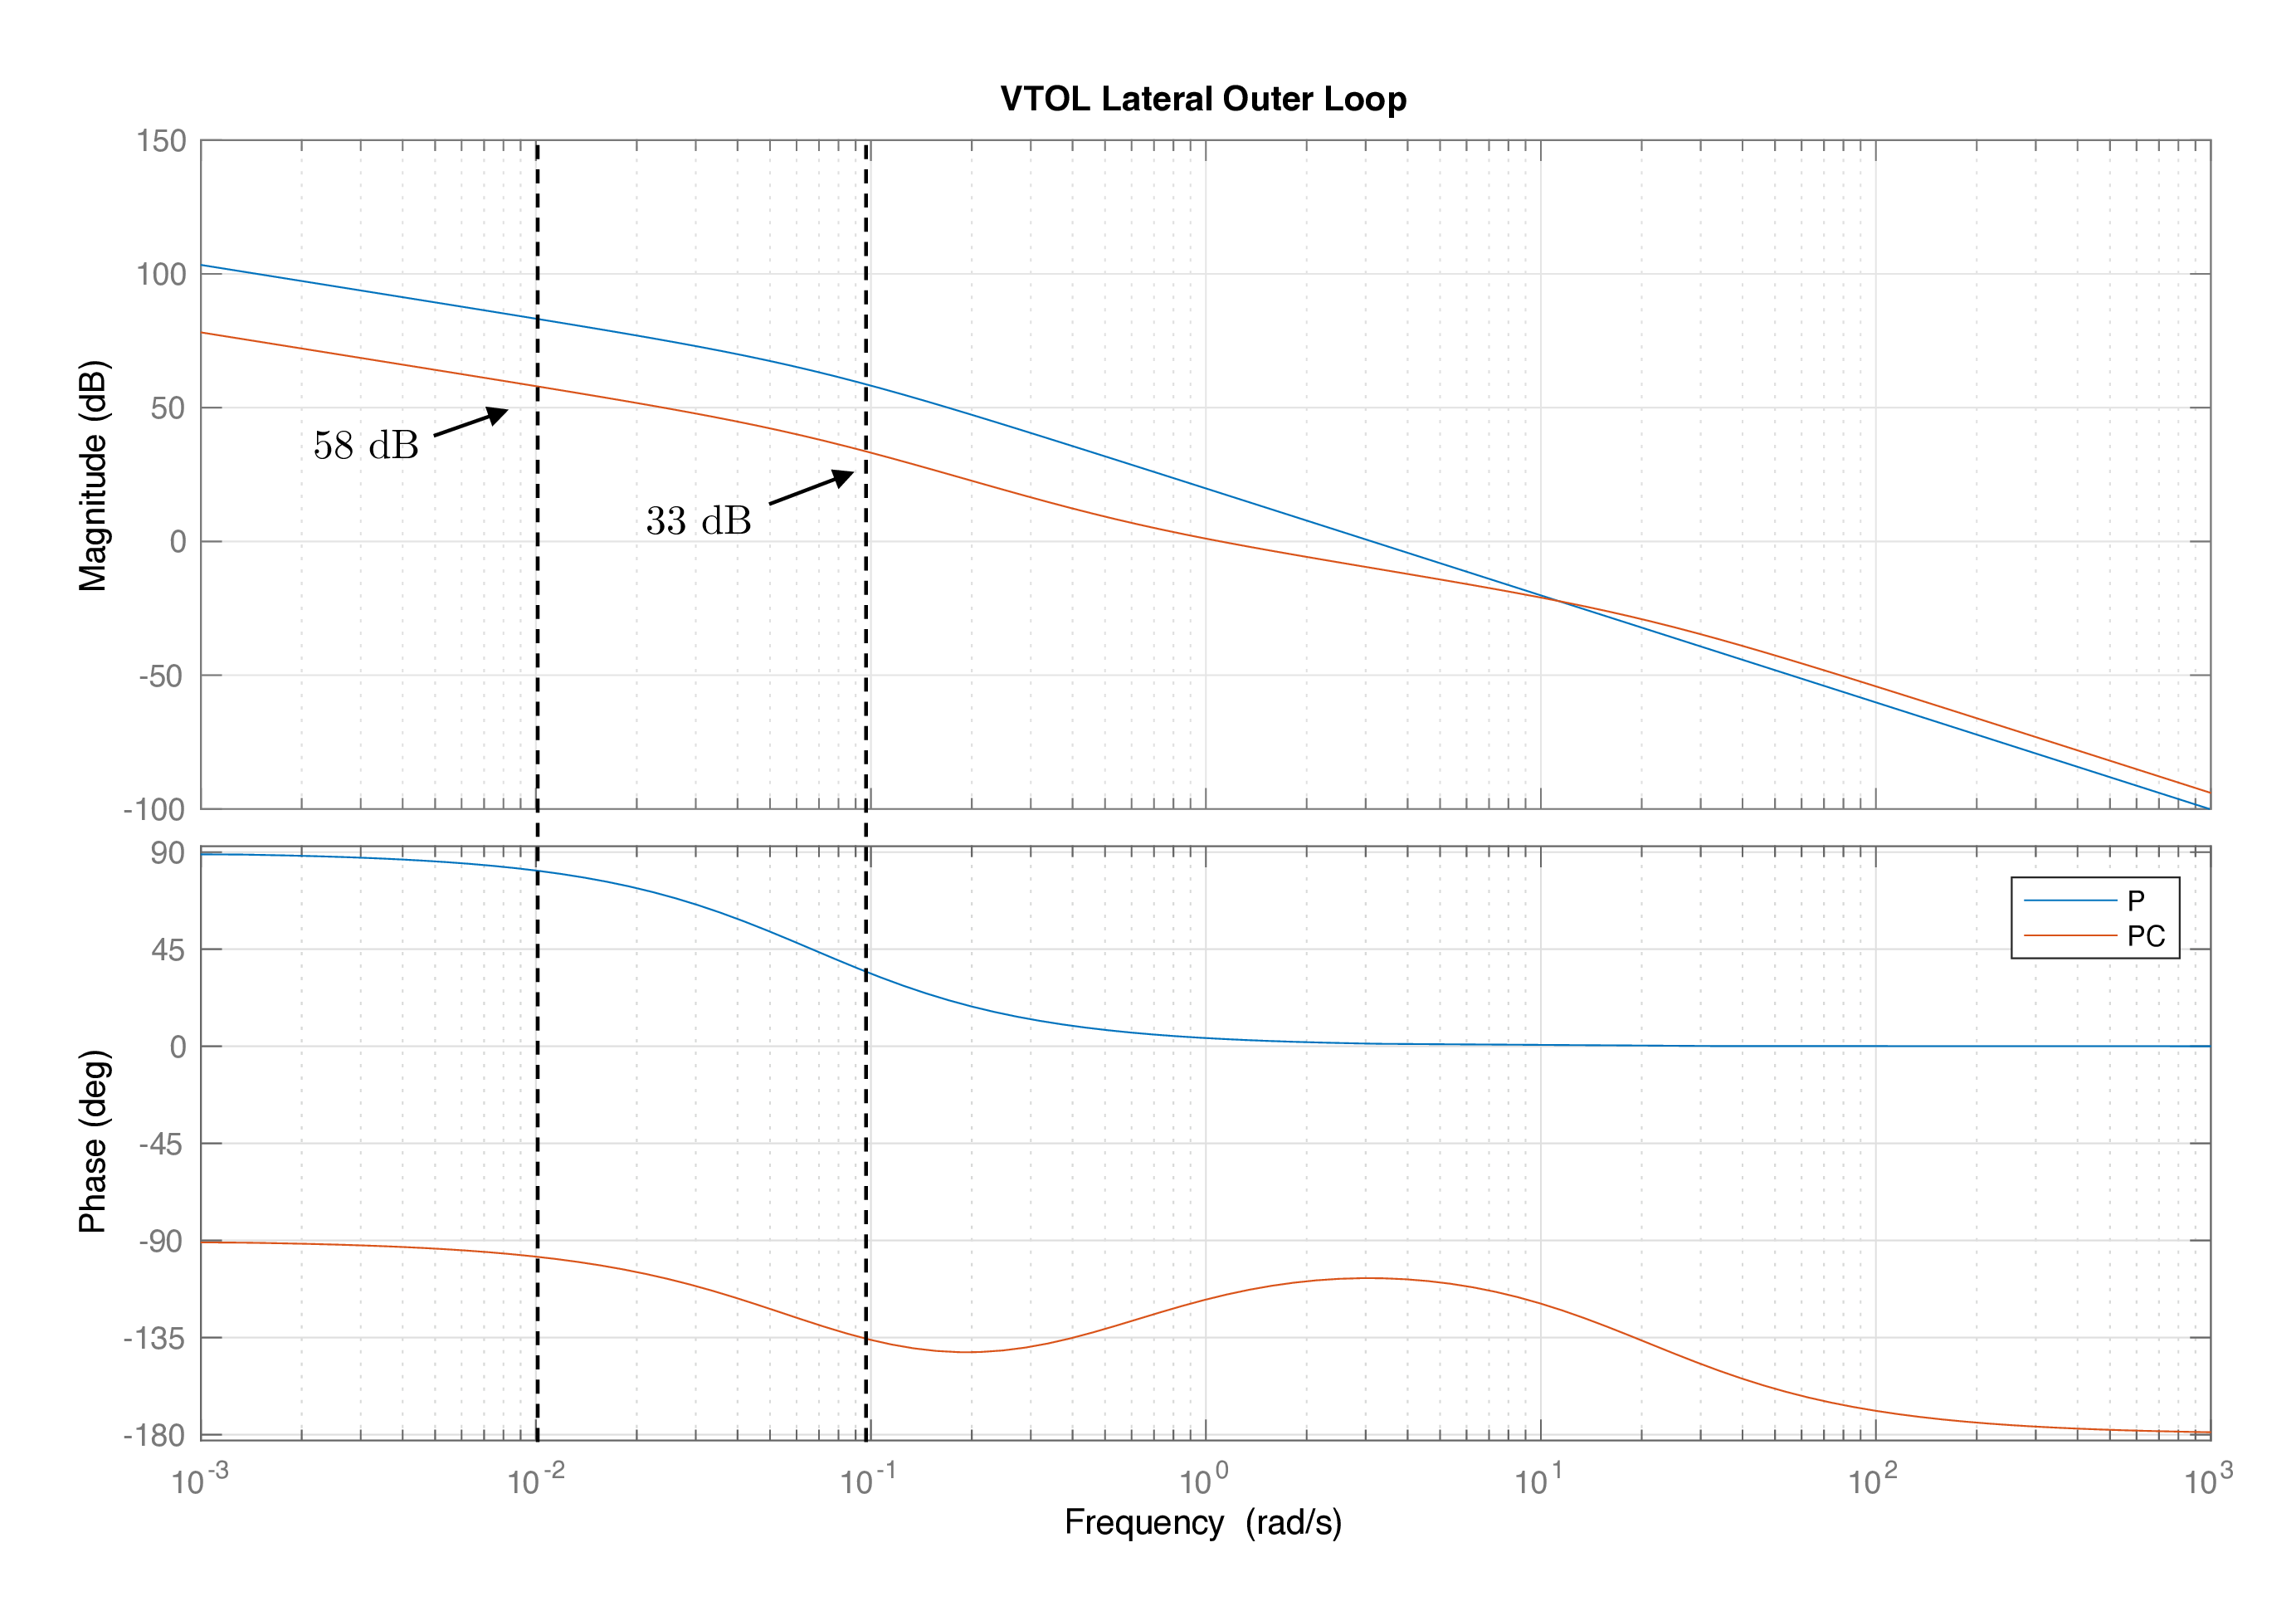
\includegraphics[width=0.95\textwidth]{6_design_studies/figures/hw_vtol_lat_bode_specs_out.pdf}
   \caption{Bode plot for lateral outer loop of the VTOL system, plant only, and under PD control.}
   \label{fig:hw_vtol_lat_bode_specs_out}
\end{figure}

{\bf (e)}
From Figure~\ref{fig:hw_vtol_lat_bode_specs_out} we see that for $\omega<\omega_r=0.1$~rad/sec, the loop gain is greater than $B_r=33$~dB.  Therefore, the tracking error satisfies
\[
\abs{e(t)}\leq 10^{-33/20}\abs{r(t)} =0.0224 \abs{r(t)},
\]
which implies that tracking accuracy is to within $2.24$\%.

{\bf (f)}
For $\omega\leq\omega_{d_{out}}\leq 0.01$~rad/sec, we see from Figure~\ref{fig:hw_vtol_lat_bode_specs_out} that $B_{d_{out}} = 58$~dB.  Therefore, $\gamma_{d_{in}} = 10^{-58/20} = 0.0013$, which implies that $0.13$\% of the output disturbance will show up in the output signal.

